\documentclass[11pt,twocolumn]{article}
\usepackage[letterpaper,hmargin=1.0in,vmargin=1.0in]{geometry}
\usepackage{url}
\usepackage{amsmath}
\usepackage{graphicx}
\newcommand\Path{\mathcal{P}}
\setlength{\columnsep}{0.5in}

\begin{document}
\title{A Statistical Study of Signposting in Pliny's Epistles}

\author{
  Martin Kellogg\\
  \texttt{mjk6zt@virginia.edu}
}

\maketitle

\iffalse
(*
 * Copyright (c) 2015, 
 *  Martin Kellogg          <mjk6zt@cs.virginia.edu>
 * All rights reserved.
 * 
 * Redistribution and use in source and binary forms, with or without
 * modification, are permitted provided that the following conditions are
 * met:
 *
 * 1. Redistributions of source code must retain the above copyright
 * notice, this list of conditions and the following disclaimer.
 *
 * 2. Redistributions in binary form must reproduce the above copyright
 * notice, this list of conditions and the following disclaimer in the
 * documentation and/or other materials provided with the distribution.
 *
 * 3. The names of the contributors may not be used to endorse or promote
 * products derived from this software without specific prior written
 * permission.
 *
 * THIS SOFTWARE IS PROVIDED BY THE COPYRIGHT HOLDERS AND CONTRIBUTORS "AS
 * IS" AND ANY EXPRESS OR IMPLIED WARRANTIES, INCLUDING, BUT NOT LIMITED
 * TO, THE IMPLIED WARRANTIES OF MERCHANTABILITY AND FITNESS FOR A
 * PARTICULAR PURPOSE ARE DISCLAIMED. IN NO EVENT SHALL THE COPYRIGHT OWNER
 * OR CONTRIBUTORS BE LIABLE FOR ANY DIRECT, INDIRECT, INCIDENTAL, SPECIAL,
 * EXEMPLARY, OR CONSEQUENTIAL DAMAGES (INCLUDING, BUT NOT LIMITED TO,
 * PROCUREMENT OF SUBSTITUTE GOODS OR SERVICES; LOSS OF USE, DATA, OR
 * PROFITS; OR BUSINESS INTERRUPTION) HOWEVER CAUSED AND ON ANY THEORY OF
 * LIABILITY, WHETHER IN CONTRACT, STRICT LIABILITY, OR TORT (INCLUDING
 * NEGLIGENCE OR OTHERWISE) ARISING IN ANY WAY OUT OF THE USE OF THIS
 * SOFTWARE, EVEN IF ADVISED OF THE POSSIBILITY OF SUCH DAMAGE.
 *)
\fi

\section{Abstract}

Latin prose contains markers (or ``signposts'') that are believed to make it easier to read. In particular, the letters of Pliny are believed to be more rife with such signposts; other authors are hypothesized not to use them as often. We present an algorithm that finds such signposts in Latin text, and use it to demonstrate that Pliny and Cicero, in their collections of letters, do use these signposts at a much higher rate than other prose authors.    

\section{Introduction}
\label{sec:Intro}

The letters of Gauis Plinius Caecilius Secundus, more commonly known as Pliny the Younger, are often read by students of Latin.  It has been claimed \cite{Woodmanpm} that Pliny's letters are easier to read than comparable Latin texts due to Pliny favoring so called ``signpost'' words, which provide useful markers for the beginning reader. The primary goal of this paper is to determine whether this claim is, in fact, true.

``Signpost'' words come in pairs: first one introduces some grammatical structure, such as a clause or phrase, then the other introduces another parallel structure. Common examples of this pattern include ``ut'' and ``sic'' - ``just as x, in the same way y'' or ``cum'' and ``tum'' - ``both x and y''. These words are often learned early in a student's Latin career, and, it is assumed, allow the student to break up the sentence into its constituent parts. This paper assumes that a higher frequency of ``signpost'' words does, in fact, lead to more easily read Latin for the beginner; however, this assumption may be false (see section \ref{sec:Threats to Validity}).

Nevertheless, this paper endeavors to determine whether Pliny's prose includes more of these ``signpost'' words than the prose of other similar authors. In order to discover this, a computer analysis of the texts of both Pliny's epistles and other Roman writers (including Cicero, Seneca, Caesar, and Tacitus) is used. This analysis searches through the text and finds pairs of coordinated ``signpost'' words. We discuss this analysis in section \ref{sec:The Program}.
 
After data is collected, statistical methods are applied to determine whether the ``signpost'' words occur more or less frequently in different authors. The statistical methodology is discussed in section \ref{sec:stats}. The results of the statistical analysis are discussed in section \ref{sec:discuss}. section \ref{sec:Threats to Validity} discusses threats to the validity of our approach, section \ref{sec:related} discusses related work, section \ref{sec:Future} discusses possible future work, and the paper concludes in section \ref{sec:conclusion}.

\section{The Program}
\label{sec:The Program}

In order to determine how many times each of the signposts we consider is used in the texts considered, we use a simple computer program that operates over the text in question. The algorithm is straightforward, but it does rely on two major heuristics and a few other small assumptions. The source code for the algorithm about to be described, along with instructions on how to use it and the inputs used, are available at \cite{github}.

\subsection{Description of Algorithm}

The main part of the algorithm is the following: we start with a list of signpost pairs (for instance, ``cum'', ``tum'') and a file, which contains the text of the work we wish to collect data on. We read the file into our program and split it up by spaces so that we have a large list of all the words in the file. For each of the signposts we are considering, we make one pass through the word list. We begin reading the words one at a time, looking for the first word in the pair. Once we have found an instance of the first word, we begin a second search at the found word's location, looking for the second signpost in the pair.

It is here that we deploy our heuristics. The first heuristic concerns so called ``strong stops''. Although they are inserted by the editors, ``strong stops'' have been found to do a good job of determining where punctuation should actually go in ancient texts \cite{strongstop}. Because we do not expect signposts to span sentences, we do not look beyond ``strong stops'' when trying to find the second word of the pair. For our purposes, the ``strong stops'' conservatively only include the period and the colon; it is possible that a semicolon might be inserted reasonably between two signposted clauses.

The second heuristic we use is related to clause length: we only consider signposts that have at most eight other words between them. This limit was chosen somewhat arbitrarily, but when testing our implementation we discovered that it was sufficient in practice. To ensure the correctness of our program we tested against an index of Pliny \cite{index}, and a limit of eight removed all false negatives while minimizing false positives.

\subsection{Choice of Inputs}

We chose the following list of signposts to test, which we divide into two categories: the signposts that consist of two different words and the signposts that consist of the same word repeated multiple times. The different words: cum, tum; quidem, tamen; ut, sic; ut, ita; quidem, sed; tam, ut; ita, ut; adeo, ut. We also used the following words, repeated twice: et, vel, and aut.

We looked for these signposts in the following works:
\begin{itemize}
  \item Pliny's \textit{Epistulae}
  \item Cicero's \textit{Epistulae ad Familiares} and \textit{Epistulae ad Atticum}
  \item Seneca's \textit{Epistulae}
  \item Caesar's \textit{Bella Gallica}
  \item Tacitus' \textit{Agricola}
  \item Tacitus' \textit{Historiae}
\end{itemize}

A few brief words on the choice of texts: Pliny is here since that is the text of interest. Cicero and Seneca are the authors of the other two large, extant collections of letters, and so they were selected as well. Tacitus is contemporary with Pliny, and so is selected to control for changes in the language that might make signposting more common. Originally, we used only the \textit{Agricola}, but during the statistical analysis we discovered that it was too small for an effective sample. Therefore, we added Tacitus' \textit{Historiae} as an additional contemporary. We leave the numbers for the \textit{Agricola} for completeness. Finally, Caesar is chosen because the \textit{Bella Gallica} is generally regarded as an easier, introductory Latin text. Since we hypothesize that signposts make Latin easier to read, comparing with an ``easier'' text makes sense.

The results of the analysis can be found in Figure \ref{fig:results}. Each column of the figure represents an author, and each row represents either the total word count of the document (``Word Count'') or the number of times a particular signpost pair was found. These results are displayed graphically in figures \ref{fig:gs} through \ref{fig:ge}, which are found at the end of the text. These figures show the relative proportion of each pair of signposts, normalized by the size of each text. These data provide a glimpse of which authors favor which constructions, and are discussed further in section \ref{sec:discuss}.

\begin{figure*}[t]
  \begin{center}
    \begin{tabular}{| l || c | c | c | c | c | c |}
      \hline
      & Pliny & Seneca & Cicero & Caesar & \textit{Agricola} & \textit{Historiae}  \\ \hline \hline
      Word Count & 69896 & 122281 & 17140 & 54349 & 6842 & 51845 \\ \hline \hline
      cum, tum & 23 & 2 & 14 & 9 & 0 & 0 \\ \hline
      quidem, tamen & 19 & 9 & 1 & 1 & 0 & 0 \\ \hline
      ut, sic & 24 & 13 & 1 & 1 & 1 & 0 \\ \hline
      ut, ita & 39 & 33 & 3 & 6 & 5 & 18 \\ \hline
      quidem, sed & 18 & 46 & 2 & 3 & 1 & 7 \\ \hline
      tam, ut & 46 & 31 & 4 & 3 & 1 & 4 \\ \hline
      ita, ut & 53 & 25 & 23 & 10 & 3 & 14 \\ \hline
      adeo, ut & 14 & 17 & 1 & 4 & 1 & 12 \\ \hline \hline
      total, non-repeat & 236 & 176 & 49 & 37 & 12 & 81 \\ \hline \hline
      et, et & 389 & 653 & 124 & 174 & 48 & 257 \\ \hline
      vel, vel & 59 & 16 & 5 & 4 & 1 & 3 \\ \hline
      aut, aut & 79 & 144 & 19 & 55 & 9 & 22 \\ \hline \hline
      total, repeat & 527 & 813 & 148 & 233 & 58 & 282 \\ \hline \hline
      total & 763 & 989 & 197 & 270 & 70 & 363 \\
      \hline
    \end{tabular}
  \end{center}
  \caption{\label{fig:results}This table contains the raw results obtained by running the algorithm described in section \ref{sec:The Program}.}
\end{figure*}

\section{Statistical Methodology}
\label{sec:stats}

A cursory examination of figure \ref{fig:results} does not yield a lot of useful information. Especially due to the tremendous differences in the sizes of the texts (Seneca's letters have nearly 200 words for every one in the \textit{Agricola}!), it is necessary to control for the size of the texts when comparing the results. We also want to be able to have empirical confidence in our results. In order to attain these goals, we use an hypothesis testing scheme between population. We compare each text with Pliny's \textit{Epistulae}, testing each time whether the proportions of the words in each text that are signposts are equal. Since we expect Pliny to contain more signposts \cite{Woodmanpm}, we use an upper-sided test. This means that our null hypothesis for each pair of texts is that the frequency of signposts is the same, and that our alternate hypothesis is that Pliny has a higher frequency of signposts.

We perform a test of this kind on two different pieces of our data: the total number of signposts in each text and the total number of ``non-repeat'' signposts (i.e. those signposts which do not consist of the same word repeated twice). Although the individual numbers of each signpost are interesting, we chose to test these two particular numbers because they encompass all the information we wish to consider and they will provide us with an answer to our original research question, which asked whether Pliny used more signposts than similar writers. Originally, we intended only to use the totals, but after seeing how many more ``repeat'' signposts there were (consider that ``et...et'' appeared in Seneca nearly twice as often as all the other signposts combined) we felt that it would be prudent to test both. Consider further that all three of the ``repeat'' signposts under test here are often just used in lists of things, which are usually somewhat uninteresting grammatically. Finally, we show in section \ref{sec:plots} that the variation in individual authors on these signposts is small, and the only one of the three that has an outsize proportion in favor of one author is ``vel, vel'' (figure \ref{fig:vv}), which favors our hypothesis that Pliny uses more signposts.

We therefore run upper-sided tests between each population and Pliny, and report the results in figure \ref{fig:stats}. We report the $p$ value we found between each of the populations for each test, which indicates the probability that we made a ``type I error'', which would indicate that we had chosen to reject the null hypothesis (thus suggesting that Pliny \textit{did} contain more signposts) when in fact we should have failed to reject it (which is to say that the $p$ value represents the probability that we thought Pliny contained more signposts when he did not). It is generally agreed that a $p$ value below 0.05 is substantial evidence for the alternate hypothesis. This means that in figure \ref{fig:stats}, we can conclude that Pliny has more signposts than another author when the $p$ value between those two authors is less than 0.05. Sometimes we know that the $p$ value is very small, so we do not bother to calculate its actual value. In these cases, we say that $p \ll 0.0001$, which means that $p$ is much smaller than $0.0001$. In these cases we always reject the null hypothesis.

\begin{figure*}[t]
  \begin{center}
    \begin{tabular}{| l | c | c | c |}
      \hline
      Pair of Authors & Non-repeat or total & $p$ value & Reject? \\ \hline \hline
      Pliny and Seneca & Total & $p \ll 0.0001$ & Yes \\ \hline
      Pliny and Seneca & Non-repeat & $p \ll 0.0001$ & Yes \\ \hline
      Pliny and Cicero & Total & $p \approx 0.7389$ & No \\ \hline
      Pliny and Cicero & Non-repeat & $p \approx 0.1446$ & No \\ \hline
      Pliny and Caesar & Total & $p \ll 0.0001$ & Yes \\ \hline
      Pliny and Caesar & Non-repeat & $p \ll 0.0001$ & Yes \\ \hline
      Pliny and Tacitus's \textit{Agricola} & Total & $p \approx 0.3015$ & No \\ \hline
      Pliny and Tacitus's \textit{Agricola} & Non-repeat & $p \approx 0.0119$ & Yes \\ \hline
      Pliny and Tacitus's \textit{Historiae} & Total & $p \ll 0.0001$ & Yes \\ \hline
      Pliny and Tacitus's \textit{Historiae} & Non-repeat & $p \ll 0.0001$ & Yes \\      
      \hline
    \end{tabular}
  \end{center}
  \caption{\label{fig:stats}The results of the statistical analysis desrcibed in section \ref{sec:stats}.}
\end{figure*}

\section{Discussion}
\label{sec:discuss}

We consider both the table in figure \ref{fig:stats} and the series of graphs reproduced at the end of the paper (figures \ref{fig:gs} to \ref{fig:ge}). First we discuss the overall statistics, then we discuss the individual graphs.

\subsection{Overall results}

The results in figure \ref{fig:stats} show that Pliny does, in fact, use fewer signposts than many of the other authors to which he is compared. In particular, Pliny uses many, many more signposts than either Seneca or Caesar, which seems to support our original claim that Pliny used an unusually large number of signposts.

However, when Pliny is compared to a contemporary, his friend Tacitus, the results are more mixed. When comparing the total number of signposts in the \textit{Agricola}, it appears as if, although Pliny uses a slightly higher proportion of signposts than Tacitus, the numbers are close enough that it's difficult to be confident that the difference is not due to random variation. When we only compare using the non-repeated signposts, on the other hand, we can be reasonably confident that Pliny is in fact using more. These uncertainties, however, are probably due more to the small sample size of the \textit{Agricola}. Because it is so much shorter than the corpus of Pliny to which it is being compared, and the frequency of individual signposts among the total number of words is quite low (even when signposts are very common, they still make up a very small percentage of the whole text), our statistical test cannot give us too high a level of confidence. 

Instead, we can look at the \textit{Historiae}, a more significant work by Tacitus. When we compare this work to Pliny's letters, we can conclude firmly that the larger proportion of signposts in Pliny's work is statistically significant. Unsurprisingly, when we combine all of Tacitus' work under consideration, we get similar results to just the \textit{Historiae}, most likely due to the domination of the larger sample. From this, we can safely decide that Pliny is also using more signposts than Tacitus.

Finally, this leaves the case of Cicero's \textit{Epistulae}. Not only can we not conclude that Cicero's letters use fewer signposts than Pliny, $p$ values greater than 0.5 indicate that Cicero may actually use signposts \textit{more} than Pliny. A test of this (essentially running the same test between Pliny and Cicero in reverse, to see if we have convincing evidence that Cicero uses more signposts than Pliny) also is inconclusive. Since we do not have strong evidence that either uses more signposts than the other, we are justified in concluding that both letter-writers use signposts equally often. 

Moreover, Pliny is thought to have held Cicero in the highest regard \cite{plinycicero1} \cite{plinycicero2}. Not only were both politicians and lawyers, but also both released books of letters for publication; it is natural that we should expect the two to be similar. It is no surprise, then, that the two cannot be differentiated on the basis of signposting. To see to what degree Pliny might be modelling his letters on those of Cicero (as opposed to Cicero as a whole), we also conducted a test of the kind described above on some of Cicero's speeches against Cataline. These speeches contained much less frequent use of signposts than any of Cicero's letters. Perhaps, then, signposting is a trademark of epistolary writings? A quick glance at our results for Seneca's books of letters show that this is not the case. Rather, then, the similarity between Pliny and Cicero seems to provide further evidence for the claim that Pliny was explicitly modelling himself on Cicero. All told, Cicero and Pliny seem to stand out from the rest of the considered authors in their use of signposting.

\subsection{Individual signposts}
\label{sec:plots}

We now turn our attention to the relative representation of each signpost in each of the texts we examined. The data from which we are working is reproduced in figures \ref{fig:gs} to \ref{fig:ge} in a visual format. These graphs are produced by taking the number of times a signpost pair appears in the corpus and dividing by the number of words in that corpus (so that each corpus has equal weight). This produces a frequency, which is a nearly unreadable number (due to the large size of the corpora compared to the number of each signpost that appear); the frequency is therefore compared as a ``unitless'' quantity to the frequencies of the same signpost pair in other texts. Notably, every author excepting Caesar appears to have at least one signpost they particularly favor, compared to the other authors under consideration. Tacitus favors ``ut, ita'' in the \textit{Agricola} (figure \ref{fig:ui}) but ``adeo, ut'' in the \textit{Historiae} (figure \ref{fig:au}); Seneca favors ``quidem, sed'' (figure \ref{fig:qs}); Cicero especially prefers ``cum, tum'' and ``ita, ut'' (figures \ref{fig:ct} and \ref{fig:iu}); Pliny is partial to ``quidem tamen'' (figure \ref{fig:qt}), ``ut, sic'' (figure \ref{fig:us}), and ``vel, vel'' (figure \ref{fig:vv}); only Caesar does not dominate at least one of the plots. On the other hand, both ``et, et'' and ``aut, aut'' are not dominated by a single author, but rather show relatively even use among all (see figures \ref{fig:ee} and \ref{fig:aa}). It is primarily for this reason that we used the ``non-repeating'' comparisons in section \ref{sec:stats}. All told, these plots provide interesting information for one interested in the particulars of an author's language; however, the sample sizes on each individual signpost pair are really too small for a rigorous statistical analysis using a multi-population hypothesis test, as we have done.  

\section{Threats to Validity}
\label{sec:Threats to Validity}

Although our approach has demonstrated with a great degree of confidence that Pliny's \textit{Epistulae} do have more signposting words than most of the Latin authors under consideration, it does so with a few caveats. First, as noted in section \ref{sec:The Program}, we make a number of assumptions regarding the placement of signpost words. It is certainly possible that our heuristics, in particular with regards to the number of words in between the signposts, may be misguided. They were only tested experimentally on a single pair of signposts, and it is very possible that the results would look different if a different heuristic were applied. That said, the $p$ values we calculated on our statistics were so low on most authors (excepting, of course, Cicero) that even if we were systematically missing some signposts, we would still find that Pliny exhibited a greater number of signposts than the other considered authors.

Another possible caveat concerns our statistical approach. The approach we used (pairwise hypothesis testing) relies on the normality of the underlying population. That is to say, our approach could be compromised if the number of signpost words is not a random variable that is primarily clustered around a single mean for each author. We believe that due to the rather large sample size and the naturalness of language that our proportional test does a good job of showing that the variations we observe are not due to chance, but others have argued that normality ought not to be assumed in corpus linguistics except under particular circumstances \cite{chi2}. Nevertheless, many linguists are willing to suggest techniques similar to ours \cite{gries}, and others believe that most of the commonly used techniques are inadequate \cite{bestgen}.

We have previously noted that Cicero and Pliny are the two outliers in our data set; the two are comparable but quite different from the rest. Both corpora are books of letters; we noted earlier that Seneca's similar collection exhibited very different results, which placed it squarely amongst the other authors and not with Pliny and Cicero. Nevertheless, it is possible that Pliny and Cicero are not the exceptional writers here, but rather the use of signposts is standard in epistolatory writing and Seneca is the outlier. We have no way of testing this without additional, significant books of letters, which unfortunately are not extant; the letters of M. Cornelius Fronto may be an exception.

\section{Related Work}
\label{sec:related}

The use of computers for the analysis of classical literature dates back to the early days of computer technology. Early efforts focused on the use of computers to create word lists and concordances; this work builds on the efforts of those early pioneers \cite{early}. Once computers became somewhat more widely available, research focused on identifying the authorship of works - in particular the \textit{Historia Augusta} \cite{marriott}. Some early statistical pitfalls were discovered, and more recent work has been done to correct them \cite{sansone} \cite{purple}; we endeavor to avoid similar missteps. Some more modern research focuses on the use of similar techniques for the purposes of finding intertextuality \cite{forstall}. In computer science, the field of natural language processing (NLP) has been fueled by the increasingly outsize role of the internet in everyday life; for a summary of recent developments, see e.g. \cite{nlp}. While it appears that the rate of crossover between these exciting new techniques and classics research is slow, it is our hope that the classics community will begin to adapt these recent advances.

\section{Future Work}
\label{sec:Future}

This paper only outlines a somewhat crude beginning to a more complete investigation of this topic. We deploy a set of simple heuristics and an elementary statistical analysis, and the results we have produced seem to indicate that further work may be warranted. First, a larger collection of latin texts could be studied. An investigation could be made of whether the differences between the pair of Pliny and Cicero and the rest of the authors is in fact due to the epistolary character of their work using other, smaller collections of extant letters. We could look for other authors that use more signposts, and see if there are any interesting relationships among those that are. Second, our experimental methods could be refined. Our heuristics could be tested further empirically, and more complex statistical methods (such as the chi-squared test favored by \cite{chi2} or the entropy method used by e.g. \cite{software}. We could also examine our assumption that more signposts do make it easier for students to read the Latin; a human study could be used to address this.

\section{Conclusion}
\label{sec:conclusion}

We present an algorithm with empirically backed heuristics to identify signpost pairs in Latin prose. This algorithm combines modern computational techniques with a knowledge of the Latin grammar and structure in question to reliably identify signposts. We then use this algorithm to determine whether Pliny's \textit{Epistulae} contain more signposts than the writings of other authors, as we hypothesize. Using a combination of statistical methods and empirical data acquired with our program, we show that Pliny, on the whole, is one of the most prolific users of signposting among a selection of Latin prose authors; only he and Cicero stand out among the crowd.


\bibliographystyle{plain-title}
\bibliography{references}

\appendix
\section{Appendix A}

\begin{figure}
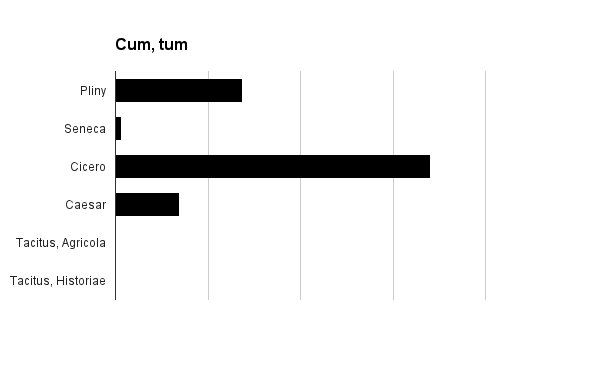
\includegraphics[width=0.5\textwidth]{cumtum.png}
\caption{\label{fig:gs}\label{fig:ct}Frequency of cum, tum}
\end{figure}

\begin{figure}
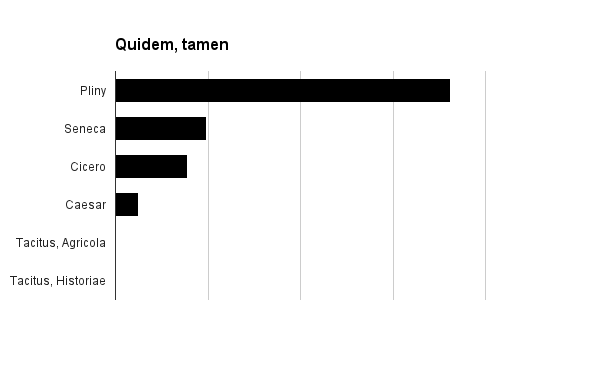
\includegraphics[width=0.5\textwidth]{quidemtamen.png}
\caption{\label{fig:qt}Frequency of quidem, tamen}
\end{figure}

\begin{figure}
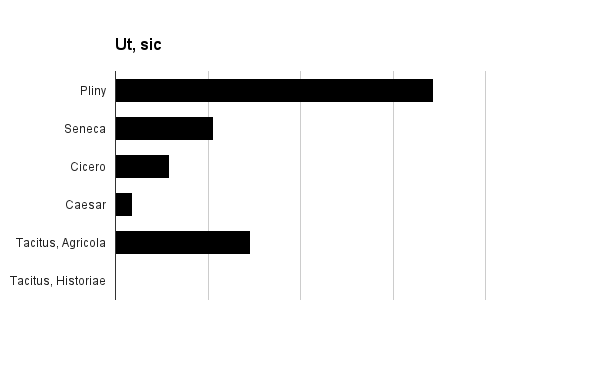
\includegraphics[width=0.5\textwidth]{utsic.png}
\caption{\label{fig:us}Frequency of ut, sic}
\end{figure}

\begin{figure}
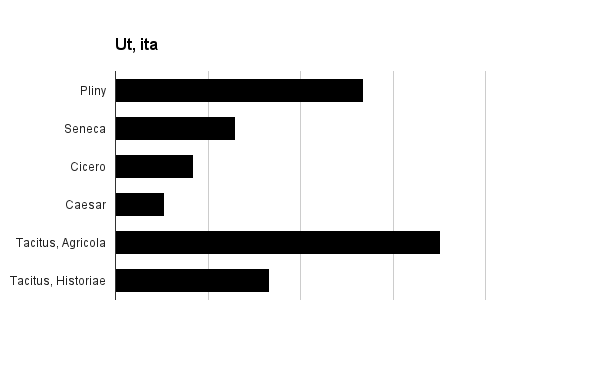
\includegraphics[width=0.5\textwidth]{utita.png}
\caption{\label{fig:ui}Frequency of ut, ita}
\end{figure}

\begin{figure}
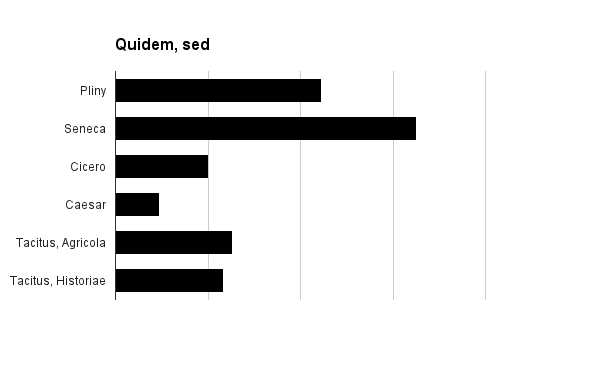
\includegraphics[width=0.5\textwidth]{quidemsed.png}
\caption{\label{fig:qs}Frequency of quidem, sed}
\end{figure}

\begin{figure}
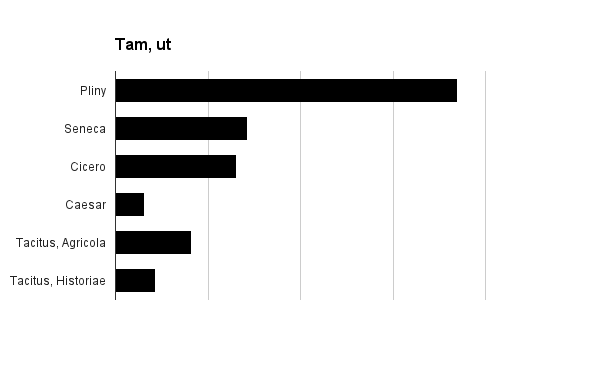
\includegraphics[width=0.5\textwidth]{tamut.png}
\caption{\label{fig:tu}Frequency of tam, ut}
\end{figure}

\begin{figure}
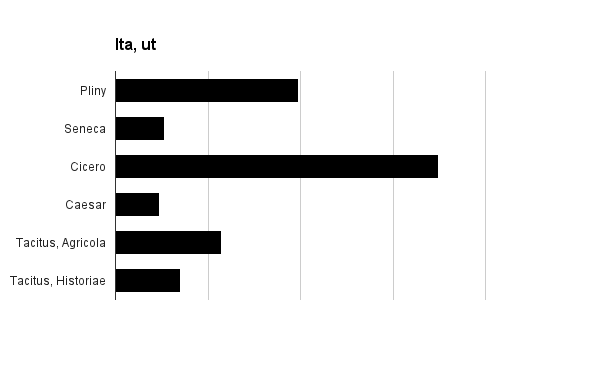
\includegraphics[width=0.5\textwidth]{itaut.png}
\caption{\label{fig:iu}Frequency of ita, ut}
\end{figure}

\begin{figure}
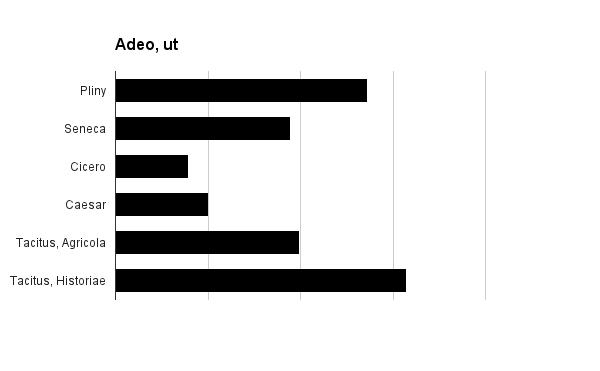
\includegraphics[width=0.5\textwidth]{adeout.png}
\caption{\label{fig:au}Frequency of adeo, ut}
\end{figure}

\begin{figure}
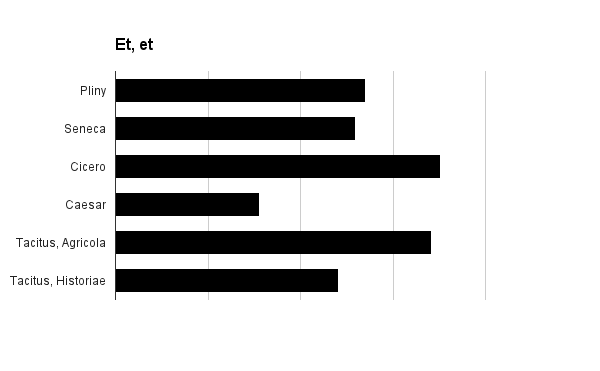
\includegraphics[width=0.5\textwidth]{etet.png}
\caption{\label{fig:ee}Frequency of et, et}
\end{figure}

\begin{figure}
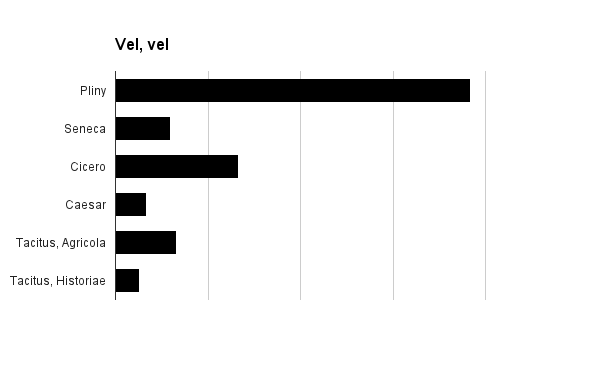
\includegraphics[width=0.5\textwidth]{velvel.png}
\caption{\label{fig:vv}Frequency of vel, vel}
\end{figure}

\begin{figure}
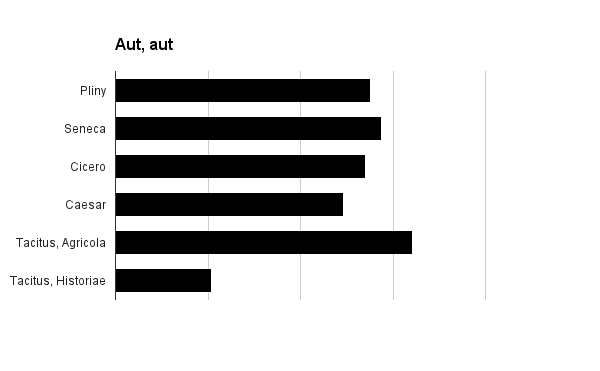
\includegraphics[width=0.5\textwidth]{autaut.png}
\caption{\label{fig:ge}\label{fig:aa}Frequency of aut, aut}
\end{figure}

\end{document}
